\chapter{Some Properties of Trees}
\label{sct_defining_clades}

\begin{figure}[t]
\centering
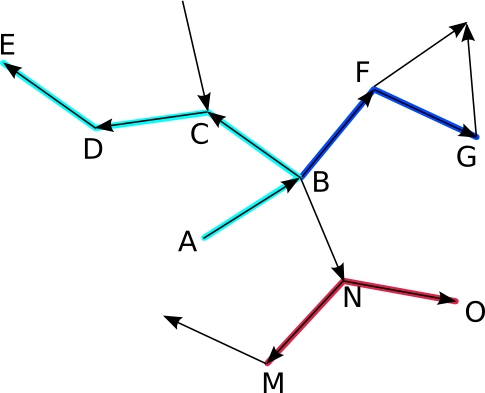
\includegraphics{oriented_graph.png}
 % oriented_graph.png: 485x393 pixel, 300dpi, 4.11x3.33 cm, bb=0 0 116 94
 \caption{An oriented graph (not a tree!), with edge orientation shown as arrows. Two paths are highlighted (cyan and blue). The cyan path starts at node A and ends at node E. Nodes B, C, D, and E are reachable from A. Node C is the direct successor of B in the cyan path; in the blue path the direct successor of B is F. The segment highlighted in red is \emph{not} a path.}
 \label{fig_oriented_graph}
\end{figure}



In the following, $T$ will be a rooted tree. We'll recall that a tree (rooted or not) is a connected, acyclic graph. By choosing one node to be the root (which we'll note $R$), and orienting all edges away from the root, we get an oriented graph. A \textit{path} along such a graph is a sequence of nodes such that there is an edge between two successive nodes, and that these nodes are ordered in the sequence as they are in the edge. The first node in the path is called the \textit{start} of the path, and the last node is its \textit{end}. We speak of a path \textit{from} the start \textit{to} the end, equivalently we say that the end is \textit{reachable} from the start. The nodes in a path are ordered: if $a$ and $b$ are in a path, then either $a$ is reachable from $b$, or $b$ is reachable from $a$, or $a = b$; furthermore if $a$ is reachable from $b$, then $b$ is \textit{not} reachable from $a$. If an edge connects $a$ to $b$, then $b$ is the \textit{direct successor} of $a$, and $a$ is the \textit{direct predecessor} of $b$
See figure {\ref{fig_oriented_graph}.

Although paths are not sets, we will (somewhat abusively, perhaps) use set notation with paths, unless there is a risk of confusion. Thus is $P$ is a path and $n$ is a node, then $n \in P$ means that $n$ is ``in'' $P$  or ``belongs to'' $P$ (strictly speaking, $n$ is reachable from the start of $P$, and the end of $P$ is reachable from $n$).

Now a few definitions - these are mostly renamings of graph-theoretical concepts, to make them more intuitive for phylogenetic trees. 

\begin{dfn}
\label{def_ancestor}
Let $a$ and $b$ be two different nodes of $T$. We say that $a$ is an \textit{ancestor} of $b$, or (equivalently) that $b$ is a \textit{descendant} of $a$, if and only if there is a path from $a$ to $b$. 
\end{dfn}

\begin{dfn}
\label{def_parent}
Let $P$ be a path in $T$, and $a, b$ two nodes in $P$ such that $b$ is the direct successor of $a$. We will call $a$ the \textit{parent} of $b$. We can say \textit{the} parent (rather than \textit{a} parent) of $b$ because i) $a$ lies on the path from $R$ to $b$ (which is unique), and ii) only one node on any path can be another node's direct predecessor. We also see that any node's parent is also its ancestor (which shouldn't be too surprising\ldots), since $b$ is reachable from $a$
\end{dfn}

\begin{dfn}
\label{def_child}
Let $P$ be a path in $T$, and $a, b$ two nodes in $P$ such that $b$ is the direct successor of $a$. We say that $b$ is a \textit{child} of $a$.
\end{dfn}

Note that a node has exactly one parent, except the root which has none. A node can have zero or more children, but we rarely ever encounter nodes with a single child. A node with no children is called a \textit{leaf}.

\begin{dfn}
\label{def_lineage}
A path that starts from the root we call a \emph{lineage}. By the definition of a rooted tree, there is always a lineage to $n$ for any node $n$, and this lineage is unique. So we can unambiguously talk of \textit{the} lineage of $n$ to mean the path from $R$ to $n$. We say that a set $L$ of nodes form a lineage if there exists $n \in L$ such that the path from $R$ to $n$ contains all and only elements of $L$.
\end{dfn}

\begin{figure}[b]
 \centering
 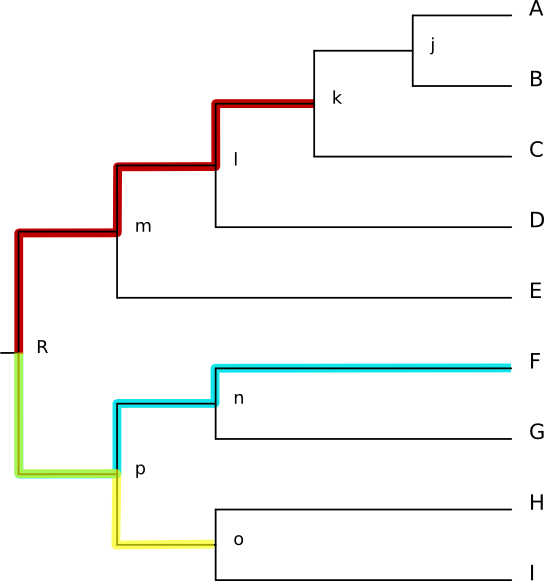
\includegraphics{prop_tree.png}
  \caption{A rooted tree}
 \label{fig_app_tree_prop}
\end{figure}

\begin{prop}
\label{prop_lineage_ancestors_equivalence}
Let $n$ be a node of $T$, and $L$ its lineage. Then all ancestors of $n$ belong to $L$, and all nodes of $L$, except $n$ itself, are ancestors of $n$.
\end{prop}

\begin{proof}

$\Rightarrow$ Let $a$ be an ancestor of $n$. By definition \ref{def_ancestor}, there is a path from $a$ to $n$. By tree properties, there is a path from $R$ to $a$. Hence $a$ belongs to the path from $R$ to $n$, which is the lineage of $n$.
\end{proof}

\noindent{}$\Leftarrow$ Let $l \neq n$ be a node in $L$. Since $L$ is the path from $R$ to $n$, $n$ is reachable from $a$, and hence $a$ is an ancestor of $n$ by definition \ref{def_ancestor}.

\begin{dfn}
If $L$ and $M$ are lineages of $T$, then the \textit{intersection}
of $L$ and $M$, noted $L \cap M$, is the set of nodes that belong to both $L$ and $M$.
\end{dfn} 

\begin{lemma}
\label{lem_ancestors_in_lineage}
Let $n$ be a node of $T$, $L$ its lineage, and $l$ a node of $L$. Then $l$'s ancestors also belong to $L$.
\end{lemma}
\begin{proof}
If $l = n$ then the ancestors of $l$ are those of $n$, which belong to $L$ by proposition \ref{prop_lineage_ancestors_equivalence}. If $l \neq n$ then let $a$ be an ancestor of $l$. By definition \ref{def_ancestor}, $l$ is reachable from $a$. By proposition \ref{prop_lineage_ancestors_equivalence}, $l$ is an ancestor of $n$ and again $n$ is reachable from $l$. Therefore, $n$ is reachable from $a$, so $a$ is an ancestor of $n$, and so belongs in $L$.
\end{proof}

\begin{lemma}
Let $L$ and $M$ be lineages of $T$, and $q \in L \cap M, q \neq R$. Then $q$'s parent also belongs to $M \cap L$.
\end{lemma}
\begin{proof}
Call $p$ the parent of $q$. $p$ is an ancestor of $q$, and since $q$ belongs to $L$ (by hypothesis), $p$ belongs to $L$ by lemma \ref{lem_ancestors_in_lineage}. By the same reasoning, $p$ belongs to $M$, therefore $p \in L \cap M$.

\end{proof}


\begin{prop}
\label{prop_lineage_intersection}
Let $L$ and $M$ be lineages of $T$. Then $L \cap M$ also forms a lineage.
\end{prop}
\begin{proof}
Let $N = L \cap M$. Because $N$ is a subset of a lineage (in fact it is a subset of at least two lineages, $L$ and $M$), its elements are ordered, so we can pick the last one and call it $n$. Now all other elements of $N$ are ancestors of $n$, so by lemma \ref{lem_ancestors_in_lineage} they belong in $L$ and in $M$. So far we have proven 
\end{proof}

\begin{prop}
In a rooted tree, you can always define a clade by specifying a single node: the clade consists of the specified node and all its descendants.
\end{prop}

\begin{prop}
In a rooted tree $T$ with unique labels and a node $n$ in $T$, it is always possible to choose two nodes $n_1$ and $n_2$ such that lca($n_1$,$n_2$) = $n$.
\end{prop}